\documentclass[tikz,border=6pt]{standalone}
\usepackage[T1]{fontenc}
\usepackage{lmodern}
\usepackage{amsmath,amssymb}
\usetikzlibrary{positioning,calc,fit}

\definecolor{inkblack}{HTML}{141416}
\definecolor{slateink}{HTML}{334155}
\definecolor{mutedgray}{HTML}{64748B}
\definecolor{navyfill}{HTML}{2B3A67}
\definecolor{plumfill}{HTML}{5B3E6B}
\definecolor{tealpill}{HTML}{E2E8F0}

\begin{document}
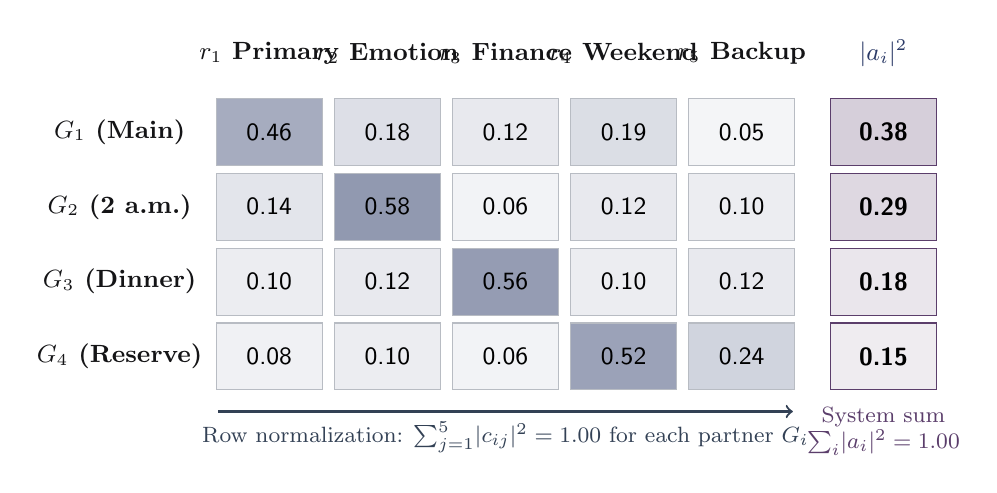
\begin{tikzpicture}[
  font=\small\sffamily,
  cell/.style={minimum width=1.35cm, minimum height=0.85cm, draw=slateink!35, anchor=center},
  hdr/.style={minimum width=1.35cm, minimum height=0.65cm, font=\bfseries\small, text=inkblack},
  rhdr/.style={minimum width=2.2cm, minimum height=0.85cm, font=\bfseries\small, text=inkblack, align=right}
]

% Column headers (Roles)
\node[hdr] (r1) at (0, 0) {$r_1$ Primary};
\node[hdr] (r2) at (1.5, 0) {$r_2$ Emotion};
\node[hdr] (r3) at (3.0, 0) {$r_3$ Finance};
\node[hdr] (r4) at (4.5, 0) {$r_4$ Weekend};
\node[hdr] (r5) at (6.0, 0) {$r_5$ Backup};
\node[hdr, text=navyfill] (ai) at (7.8, 0) {$\lvert a_i \rvert^2$};

% Matrix values (row sums = 1.00)
\def\rows{
  {1/G_1/0.46/0.18/0.12/0.19/0.05/0.38},
  {2/G_2/0.14/0.58/0.06/0.12/0.10/0.29},
  {3/G_3/0.10/0.12/0.56/0.10/0.12/0.18},
  {4/G_4/0.08/0.10/0.06/0.52/0.24/0.15}
}

% Row 1
\node[rhdr] at (-1.9, -1.0) {$G_1$ (Main)};
\node[cell, fill=navyfill!42] at (0, -1.0) {0.46};
\node[cell, fill=navyfill!16] at (1.5, -1.0) {0.18};
\node[cell, fill=navyfill!11] at (3.0, -1.0) {0.12};
\node[cell, fill=navyfill!17] at (4.5, -1.0) {0.19};
\node[cell, fill=navyfill!5]  at (6.0, -1.0) {0.05};
\node[cell, fill=plumfill!25, draw=plumfill] at (7.8, -1.0) {\textbf{0.38}};

% Row 2
\node[rhdr] at (-1.9, -1.95) {$G_2$ (2 a.m.)};
\node[cell, fill=navyfill!13] at (0, -1.95) {0.14};
\node[cell, fill=navyfill!52] at (1.5, -1.95) {0.58};
\node[cell, fill=navyfill!6]  at (3.0, -1.95) {0.06};
\node[cell, fill=navyfill!11] at (4.5, -1.95) {0.12};
\node[cell, fill=navyfill!9]  at (6.0, -1.95) {0.10};
\node[cell, fill=plumfill!20, draw=plumfill] at (7.8, -1.95) {\textbf{0.29}};

% Row 3
\node[rhdr] at (-1.9, -2.90) {$G_3$ (Dinner)};
\node[cell, fill=navyfill!9]  at (0, -2.90) {0.10};
\node[cell, fill=navyfill!11] at (1.5, -2.90) {0.12};
\node[cell, fill=navyfill!50] at (3.0, -2.90) {0.56};
\node[cell, fill=navyfill!9]  at (4.5, -2.90) {0.10};
\node[cell, fill=navyfill!11] at (6.0, -2.90) {0.12};
\node[cell, fill=plumfill!13, draw=plumfill] at (7.8, -2.90) {\textbf{0.18}};

% Row 4
\node[rhdr] at (-1.9, -3.85) {$G_4$ (Reserve)};
\node[cell, fill=navyfill!7]  at (0, -3.85) {0.08};
\node[cell, fill=navyfill!9]  at (1.5, -3.85) {0.10};
\node[cell, fill=navyfill!6]  at (3.0, -3.85) {0.06};
\node[cell, fill=navyfill!47] at (4.5, -3.85) {0.52};
\node[cell, fill=navyfill!22] at (6.0, -3.85) {0.24};
\node[cell, fill=plumfill!10, draw=plumfill] at (7.8, -3.85) {\textbf{0.15}};

% Annotations
\draw[->, thick, slateink] (-0.65, -4.55) -- (6.65, -4.55)
  node[midway, below, font=\footnotesize\color{slateink}] {Row normalization: $\sum_{j=1}^{5} \lvert c_{ij}\rvert^2 = 1.00$ for each partner $G_i$};
\node[font=\footnotesize\color{plumfill}, align=center] at (7.8, -4.80) {System sum\\$\sum_i \lvert a_i\rvert^2 = 1.00$};

\end{tikzpicture}
\end{document}
